\documentclass[a4paper,11pt]{article} % preambuła
\usepackage[polish]{babel}
\usepackage[utf8]{inputenc} % utf8, cp1250
\usepackage{pslatex}
\usepackage[T1]{fontenc}
\usepackage{times}
\usepackage{geometry}
\usepackage{algorithm}
\usepackage{graphicx}
\usepackage{xcolor}
\usepackage{wrapfig}
\usepackage{amsmath}
\usepackage{subcaption}
\usepackage{algpseudocode}
\usepackage{pgfplots}
\newgeometry{tmargin=1.5cm, bmargin=1.5cm, lmargin=1.5cm, rmargin=1.5cm}

\begin{document}
\section{Omów prawa Kirchhoffa.}
I prawo Kirchoffa (prądowe prawo Kirchoffa) mówi, że w węzłach sieci, tzn. w punktach wspólnych dla trzech lub więcej przewodów, algebraiczna suma natężeń prądów wpływających musi być równa zeru. A więc suma natężeń prądów wpływających do węzła jest równa sumie natężeń prądów wypływających z tego węzła.

II prawo Kirchoffa (napięciowe prawo Kirchoffa) mówi, że suma różnic potencjałów obliczonych kolejno wzdłuż zamkniętej pętli sieci (tzw. oczka) - tzn. drogi, która rozpoczyna się i kończy w tym samym węźle - równa się zeru.

\section{Wyprowadź wzory na opór zastępczy dla połączenia szeregowego i równoległego
dwóch oporników R1 i R2 .
}
Dla połączenia szeregowego mamy:\\
Prąd I wymuszony napięciem zasilania U wytworzy na R1 i R2 spadki napięć U1, U2. \\Z drugiego prawa Kirchoffa U = U1 + U2, więc:\\
$$R = \frac{U}{I} = \frac{U1+U2}{I} = \frac{IR1 + IR2}{I} = \frac{I(R1+R2)}{I} = R1 + R2$$

Dla połączenia równoległego mamy: \\
Prąd I wymuszony napięciem zasilania U rozpłynie się na prądy I1, I2 w gałęziach R1, R2. \\
Z pierwszego prawa Kirchoffa I = I1 + I2, więc: \\
$$R = \frac{U}{I} = \frac{U}{I1+I2} = \frac{U}{\frac{U}{R1}+\frac{U}{R2}} = \frac{U}{U(\frac{1}{R1}+\frac{1}{R2})} = \frac{1}{\frac{1}{R1}+\frac{1}{R2}} $$
Zatem :
$$\frac{1}{R} = \frac{1}{R1} + \frac{1}{R2}$$

\section{Co to jest opór właściwy i przewodność właściwa? Od czego zależy opór
danego odcinka drutu przewodzącego? }
Opór właściwy - wielkość charakteryzująca materiały pod względem przewodnictwa elektrycznego. Oznaczana jako $ \rho$. Jednostka oporu właściwego to om $\cdot$ metr [$\Omega \cdot m$].

Przewodność właściwa - wiąże gęstość prądu elektrycznego w materiale z natężenie, pola elektrycznego powodującego przepływ tego prądu:
$$\vec{j} = \sigma \vec{E}$$
$\vec{j}$ - gęstość prądu elektrycznego\\
$\vec{E}$ - natężenie pola elektrycznego.

Wartość oporu zależy od długości przewodnika oraz pola przekroju poprzecznego. Im dłuższy przewodnik, tym większy opór. Im większe pole, tym mniejszy opór.

\section{Omów zależność oporności elektrycznej metali od temperatury. 
}
Zależność oporności od temperatury jest dla większości metali w przybliżeniu liniowa i dla szerokiego przedziału temperatur prawdziwy jest wzór:
$$ R_T = R_0(1+\alpha \cdot \Delta T)$$
gdzie:

$R_{T}$  – oporność w temperaturze $T$  [$\Omega$],\\
$R_{0}$  – oporność w temperaturze odniesienia $T_{0}$  [$\Omega$],\\
$\alpha$  – temperaturowy współczynnik oporności [$K^{-1}$],\\
$\Delta T$  – zmiana temperatury równa $T-T_{0}$  [$K$].

\section{Narysuj schemat układu dla mostka Wheatstone’a i wyprowadź wzór na
wartość nieznanego oporu dla mostka zrównoważonego.}
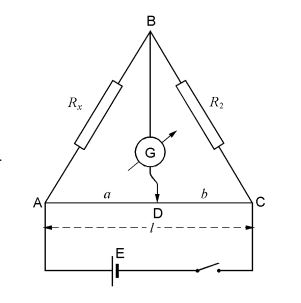
\includegraphics[scale=1]{mostek.jpg}
\\
Gdy mostek jest zrównoważony $I_{BD} = 0$ więc przyjmując $I$ jako natężenie prądu płynącego z ogniwa i korzystając z praw kirchoffa możemy utworzyć równania
$$I_{AB} + I_{AD} - I = 0$$
$$I_{AB} = I_{BC} $$
$$ I_{AD} = I_{DC} $$
z tego 
$$I_{AB}R_x = I_{AD}R_{AD}$$
$$I_{BC}R_2 = I_{DC}R_{DC}$$
$$\frac{R_x}{R_{AD}} = \frac{I_{AD}}{I_{AB}} \hspace{10pt} \frac{R_2}{R_{DC}} = \frac{I_{DC}}{I_{BC}} \hspace{10pt} \frac{R_2}{R_{DC}} = \frac{I_{AD}}{I_{AB}}$$
$$\frac{R_x}{R_{AD}} = \frac{R_2}{R_{DC}} \hspace{10pt} R_x = R_2 \frac{R_{AD}}{R_{DC}}$$
$$R_{AD} = \rho \frac{a}{S} \hspace{10pt} R_{DC} = \rho \frac{b}{S} \hspace{10pt}\text{gdzie S to przekrój drutu a } \rho \text{ to oporność właściwa materiału drutu}$$
z tego
$$ \frac{R_{AD}}{R_{DC} = \frac{a}{b}} = \frac{a}{l-a}$$
ostatecznie
$$R_x = R_2\frac{a}{l-a}$$
\section{Udowodnij, że opór zastępczy dwóch oporników połączonych równolegle
jest mniejszy od oporu mniejszego z nich.}

Dla dwóch oporników mamy:\\
$R1$ i $R2$\\
$\frac{1}{R_z} = \frac{1}{R1} + \frac{1}{R2}$ dla połączenia równoległego odwrotność oporu zastępczego = sumie odwrotności oporów składowych czyli:\\ po sprowadzeniu do wspólnego mianownika $R1 \cdot R2$ \\
$\frac{1}{R_z}= \frac{R1 + R2}{R1R2}$\\
$Rz = \frac{R1R2}{R1 + R2}$\\
Przykład: 
$$R1 = 3 \Omega , R2 = 6 \Omega$$
$$R_z = \frac{3\cdot6}{3+6} \Omega = 2 < R1$$

\section{Zdefiniuj i omów pojęcia natężenia prądu elektrycznego oraz ładunku. Podaj
definicje odpowiadających im jednostek.}
Natężenie prądu elektrycznego to wielkość fizyczna charakteryzująca przepływ prądu elektrycznego zdefiniowana jako stosunek wartości ładunku elektrycznego przepływającego przez wyznaczoną powierzchnię do czasu przepływu ładunku.
$$ I = \frac{dq}{dt}$$\\
gdzie:\\
$I$ - natężenie prądu elektrycznego\\
$dg$ - zmiana ładunku równoważna przepływającemu ładunkowi\\
$dt$ - czas przepływu ładunku.\\
Jednostka to amper [$1A = \frac{1C}{s}$]. Jeden amper odpowiada prądowi przenoszącemu w ciągu jednej sekundy ładunek jednego kulomba.

Ładunek elektryczny ciała jest podstawową cechą materii. Wszelka znana jej postać musi występować w jednym z trzech stanów: dodatni, obojętny, ujemny. Jednostką ładunku elektrycznego jest kulomb. 1 kulomb (1 C) to ładunek elektryczny przenoszony w czasie 1 sekundy (1 s) przez prąd o natężeniu wynoszącym 1 amper (1 A).

\section{Zdefiniuj i omów pojęcia napięcia oraz oporu elektrycznego. Podaj definicje
odpowiadających im jednostek.}
Napięcie elektryczne - różnica potencjałów elektrycznych między dwoma punktami obwodu elektrycznego. Jest to stosunek pracy wykonanej przeciwko polu, podczas przenoszenia ładunku elektrycznego między punktami, dla których określa się napięcie, do wartości tego ładunku.
$$ U_{AB} = \phi_B - \phi_A = \frac{W_{A\rightarrow B}}{q}$$
Jednostką napięcia jest wolt. 1 wolt (1 V) jest różnicą potencjałów elektrycznych pomiędzy dwoma punktami przewodu liniowego, w którym płynie niezmieniający się prąd o natężeniu jednego ampera (1 A). 
$$1V = \frac{1W}{1A} = \frac{1J}{1C} = \frac{1kgm^2}{1As^3}$$

Opór elektryczny - wielkość charakteryzująca relację między napięciem a natężeniem prądu elektrycznego w obwodach prądu stałego wyrażona wzorem: 
$$R = \frac{U}{I}$$
Jednostką oporu jest om. 1 om to opór elektryczny istniejący pomiędzy dwoma punktami przewodu, gdy niezmienna różnica potencjałów jednego wolta (1 V) działająca między tymi dwoma punktami wywołuje w tym przewodzie prąd o natężeniu jednego ampera (1 A).
$$1 \Omega = \frac{1V}{1A} = \frac{1kgm^2}{s^3A^2}$$

\section{Jak stwierdzić, że dwie wielkości A i B obarczone niepewnościami u(A)
oraz u(B) są sobie równe w granicach błędu? }
Jeśli do dyspozycji mamy dwie wartości zmierzone, $y1, y2$ oraz ich niepewności standardowe $u(y1), u(y2)$, to zgodnie z prawem przenoszenia niepewności różnica $y1-y2$ posiada niepewność równą sumie geometrycznej $u(y1), u(y2)$. \\
Zatem niepewność rozszerzona wynosi
$$ U(y1-y2) = k\sqrt{(u(y1))^2 +(u(y2))^2}$$
Wyniki pomiaru uważamy za zgodne ze sobą, jeżeli $|y1-y2| < U(y1-y2)$.
\end{document}